
\de{ĐỀ THI GIỮA HỌC KỲ II NĂM HỌC 2022-2023}{THPT Hùng Vương}

\begin{bt}%[0T7Y2-1]%[Dự án đề kiểm tra HKII NH22-23-Phạm Duy Phương]%[GK2-Trường THPT Hùng Vương]
	\immini{
	Dựa vào đồ thị hàm số bậc hai $y=f(x)=ax^2+bx+c$ ($a\ne 0$) đã cho, hãy nêu tập nghiệm của bất phương trình $f(x)\ge 0$.
}{
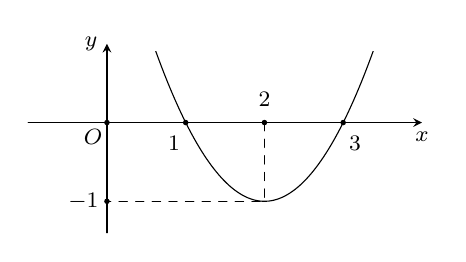
\begin{tikzpicture}[scale=1,>=stealth, font=\footnotesize, line join=round, line cap=round]
	\def\a{1} \def\b{-4} \def\c{3} % Hệ số
	\def\xmin{-1} \def\xmax{4}
	\def\ymin{-1.4} \def\ymax{1}	
	%\draw[color=gray!50,dashed] (\xmin,\ymin) grid (\xmax,\ymax);	
	\draw[->] (\xmin,0)--(\xmax,0) node [below]{$x$};
	\draw[->] (0,\ymin)--(0,\ymax) node [left]{$y$};
	\fill (0,0) circle (1pt) node[shift={(-135:2.5mm)}]{$O$};
	\clip (\xmin+0.1,\ymin+0.1) rectangle (\xmax-0.5,\ymax-0.1);
	\draw[smooth,samples=300] plot(\x,{\a*(\x)^2+\b*(\x)+\c});
	\foreach \s/\t in {1/-120,2/90,3/-60}%Trục Ox
	\fill (\s,0) circle (1pt) node[shift={(\t:3mm)}]{$\s$};
	\foreach \p/\r in {-1/180}%Trục Oy
	\fill (0,\p) circle (1pt) node[shift={(\r:3mm)}]{$\p$};
	\draw[dashed] (2,0)|-(0,-1);
\end{tikzpicture}
}
	\loigiai{
		Dựa vào đồ thị hàm số, $f(x) \ge 0$ khi và chỉ khi $x \le 1 $ hoặc $x \geq 3$.\\
		Tập nghiệm của bất phương trình là $(-\infty;1]\cup [3;+\infty)$.
	}
\end{bt}
\begin{bt}%[0T7B3-2]%[Dự án đề kiểm tra HKII NH22-23-Phạm Duy Phương]%[GK2-Trường THPT Hùng Vương]
	Giải các phương trình sau
	\begin{listEX}[2]
		\item $\sqrt{x^2-x-2}=\sqrt{2x^2+x-1}$.
		\item $\sqrt{2x^2-6x+4}-x+2=0$.
	\end{listEX}
	\loigiai{
		\begin{enumerate}
			\item Ta có
			\allowdisplaybreaks\begin{eqnarray*}
				& &\sqrt{x^2-x-2}=\sqrt{2x^2+x-1}\\
				&\Rightarrow&x^2-x-2=2x^2+x-1\\
				&\Leftrightarrow& -x^2-2x-1=0\\
				&\Leftrightarrow& x=-1.
			\end{eqnarray*}
			Thay $x=-1$ vào phương trình đã cho, ta được mệnh đề đúng.\\
			Vậy nghiệm của phương trình đã cho là $x=-1$.
			\item Ta có
			\allowdisplaybreaks\begin{eqnarray*}
				& &\sqrt{2x^2-6x+4}-x+2=0\\
				&\Rightarrow& \sqrt{2x^2-6x+4}=x-2\\
				&\Leftrightarrow& 2x^2-6x+4=(x-2)^2\\
				&\Leftrightarrow& 2x^2-6x+4=x^2-4x+4\\
				&\Leftrightarrow& x^2-2x=0\\
				&\Leftrightarrow& \hoac{&x=0\\&x=2.}
			\end{eqnarray*}
			Thay lần lượt các giá trị trên vào phương trình đã cho, ta thấy chỉ có $x=2$ thỏa mãn.\\
			Vậy nghiệm của phương trình đã cho là $x=2$.
		\end{enumerate}
	}
\end{bt}
\begin{bt}%[0T7K2-1]%[Dự án đề kiểm tra HKII NH22-23-Phạm Duy Phương]%[GK2-Trường THPT Hùng Vương]
	Tìm giá trị của tham số $m$ để $2x^2-(m-4)x+m-4>0$ với mọi $x$ thuộc $\mathbb{R}$.
	\loigiai{
		Bất phương trình $2x^2-(m-4)x+m-4>0$ đúng với mọi $x$ thuộc $\mathbb{R}$ khi và chỉ khi
		\begin{eqnarray*}
			& &\Delta=(m-4)^2-4\cdot 2\cdot (m-4)<0\quad (\text{vì }a=2>0)\\
			&\Leftrightarrow& m^2-8m+16-8m+32<0\\
			&\Leftrightarrow& m^2-16m+48<0\\
			&\Leftrightarrow& 4<m<12.
		\end{eqnarray*}
	Vậy các giá trị của $m$ thoả mãn yêu cầu đề bài là $m \in \left(4;12\right)$.
	}
\end{bt}
\begin{bt}%[0T9B2-4]%[0T9B2-2]%[Dự án đề kiểm tra HKII NH22-23-Phạm Duy Phương]%[GK2-Trường THPT Hùng Vương]
	Trong mặt phẳng tọa độ $Oxy$
	\begin{enumerate}
		\item Viết phương trình tham số của đường thẳng đi qua hai điểm $A(3;-2)$, $B(1;5)$.
		\item Viết phương trình tổng quát của đường thẳng $\Delta$ đi qua điểm $E(4;7)$ và song song đường thẳng $d\colon x-5y+3=0$.
		\item Tính số đo của góc giữa hai đường thẳng $d_1$ và $d_2$ biết
		$$d_1\colon 2x-4y+2022=0;\qquad d_2\colon 6x-2y-2023=0.$$
	\end{enumerate}
	\loigiai{
		\begin{enumerate}
			\item Đường thẳng qua $A$, $B$ nhận một véc-tơ chỉ phương là $\vec{a}=\vec{AB}=(-2;7)$.\\
			Phương trình tham số của đường thẳng là
			$$\heva{&x=3-2t\\&y=-2+7t.}$$
			\item Đường thẳng $\Delta$ song song với đường thẳng $d\colon x-5y+3=0$ có phương trình
			$$x-5y+c=0\qquad (c\ne 3).$$
			Mà $\Delta$ đi qua $E(4;7)$ suy ra
			$$4-5\cdot 7+c=0 \Leftrightarrow c=31\ (\text{thỏa mãn}).$$
			Vậy phương trình đường thẳng $\Delta$ là $x-5y+31=0$.
			\item 
			$d_1$ và $d_2$ có véc-tơ pháp tuyến lần lượt là $\vec{n_1}=(2;-4)$ và $\vec{n_2}=(6;-2)$. Ta có
			$$\cos \left(d_1,d_2\right)=\dfrac{|2\cdot 6+(-4)\cdot (-2)|}{\sqrt{2^2+(-4)^2}\cdot \sqrt{6^2+(-2)^2}}=\dfrac{\sqrt{2}}{2}.$$
			Vậy góc giữa đường thẳng $d_1$ và $d_2$ là $45^\circ$.
		\end{enumerate}
	}
\end{bt}
\begin{bt}%[0T9K2-7]%[Dự án đề kiểm tra HKII NH22-23-Phạm Duy Phương]%[GK2-Trường THPT Hùng Vương]
	Trong một khu vực bằng phẳng, ta lấy hai xa lộ vuông góc với nhau làm hai trục tọa độ của hệ trục tọa độ $Oxy$ và mỗi đơn vị độ dài trên trục tung ứng với $1$ km. Cho biết với hệ tọa độ vừa chọn thì một trạm viễn thông $S$ có tọa độ $(5;10)$. Một người đang gọi điện thoại di động trên chiếc xe ô tô chạy trên đoạn cao tốc có dạng một đường thẳng $\Delta$ có phương trình $4x-3y-5=0$. Tính khoảng cách ngắn nhất giữa người đó và trạm viễn thông $S$.
	\loigiai{
		Khoảng cách ngắn nhất giữa người đó và trạm viễn thông $S$ chính là khoảng cách từ $S$ đến đường thẳng $\Delta$.\\
		Ta có
		$$\mathrm{d}(S;\Delta)=\dfrac{|4\cdot 5-3\cdot 10-5|}{\sqrt{4^2+(-3)^2}}=3.$$
		Vậy khoảng cách ngắn nhất giữa người đó và trạm viễn thông $S$ là $3$ km.
	}
\end{bt}

